\documentclass[10pt,a4paper]{article}
\usepackage[utf8]{inputenc}
\usepackage{amsmath}
\newcommand{\RomanNumeralCaps}[1]
    {\MakeUppercase{\romannumeral #1}}
\usepackage{amsfonts}
\usepackage{amssymb}
\usepackage{float}
\usepackage{verbatim}
\usepackage{listings}
\usepackage{hyperref}
\usepackage{pbox}
\usepackage{graphicx}
\usepackage[]{algorithm2e}
%bibliography packages, bibliography files are plain text files marked .bib
%... in the same directory as the .tex file.
\usepackage[nottoc,numbib]
{tocbibind}
\usepackage{cite}
\usepackage{braket}
\usepackage{color} %red, green, blue, yellow, cyan, magenta, black, white
\definecolor{mygreen}{RGB}{28,172,0} % color values Red, Green, Blue
\definecolor{mylilas}{RGB}{170,55,241}
\usepackage{amsmath}
\usepackage{graphicx}
\graphicspath{{C:/Users/adria/Pictures/FYS3150/}}
\author{Adrian Martinsen Kleven, Simon Schrader}
\title{Project 5}

\lstset{
 	language =C++,
    frame=tb, % draw a frame at the top and bottom of the code block
    tabsize=4, % tab space width
    showstringspaces=false, % don't mark spaces in strings
    numbers=left, % display line numbers on the left
    commentstyle=\color{green}, % comment color
    keywordstyle=\color{blue}, % keyword color
    stringstyle=\color{red} % string color
}
\setlength{\columnsep}{10mm}
%\setlength{\tabcolsep}{18pt}
%\renewcommand{\arraystretch}{1.5}

\begin{document}

\part*{-Project 5 - FYS3150/FYS4150-
}
{\large \textbf{Quantum Monte Carlo of confined electrons}}\\
{\large By Simon Schrader (4150), Adrian Kleven (3150) - autumn 2019
}
\tableofcontents

\listoffigures
\listoftables


\clearpage

\section{Abstract}
Most quantum mechanical systems lack analytical solutions to the Schroedinger equation, so finding algorithms for approximating solutions is important. We explored the viability of the variational Monte Carlo method in approximating a simple quantum mechanical system. Using as the working example, two electrons in a three- dimensional harmonic oscillator potential, approximating the ground state energy, kinetic and potential energy for which there are known solutions\cite{Project2}, as well as the relative distance between electrons.\\
For small oscillator frequencies ($\omega$), the choice of trial wave function had a big impact on the accuracy of the energy expectation value, with \eqref{2ndtrialwavefunction} giving $15\%$ lower energy than \eqref{1sttrialwavefunction}, simply by the addition of the Jastrow factor \eqref{jastrow}, indicating that the inclusion of said factor is important to the accuracy of the model.\\Compared to eigenvalue solvers, as showcased in our earlier article \cite{Project2}, this stochastic method gives results $5\%$ and $6\%$ higher than the analytical results for the ground state energy depending on the trial wave function used,  making it an overall worse approximation for this system, with some caveats however. By using the variational method, our result is guaranteed to be an upper bound for the expectation value, which is in itself an incredibly useful result. In addition, the method of VMC scales more easily for more involved systems.

\section{Introduction}
The purpose of this article is to apply the Variational Monte Carlo (VMC) method to two electrons in a quantum dot, modelled by a 3- dimensional harmonic oscillator potential. This is in order to evaluate their ground state energy, relative distance, and the expectation values of their kinetic and potential energies.\\In order to benchmark the results of this method, we are comparing the results of the ground state energy with analytical solutions for specific harmonic oscillator frequencies (henceforth $\omega$) as found in M. Taut's \cite{PhysRevA.48.3561} and our previous article \cite{Project2} on the topic of electron confinement in 3- dimensional harmonic oscillator potentials.\\\\The idealized Hamiltonian used in this article, models the Coulombic interaction between electrons and the 3- dimensional harmonic oscillator potential: 
\begin{equation}
  \label{eq:finalH}
  \hat{H}=\sum_{i=1}^{N} \left(  -\frac{1}{2} \nabla_i^2 + \frac{1}{2} \omega^2r_i^2  \right)+\sum_{i<j}\frac{1}{r_{ij}}
\end{equation}
\cite{Problem_set_5} with $r_{ij}$ being the distance between electrons $i$ and $j$ with position moduli $r_i$ and $r_j$ respectively. The natural units ($\hbar = c = e = m_e =1$) are used, and energy is given in atomic units. \\\\The VMC method is implemented using C++ (see list of programs: \ref{Listofprograms}).
\section{Methods}
The VMC method is a brute force method that consists in part of a random walker, individually moving the position of the two electrons and accepting or rejecting moves in accordance with the metropolis algorithm using the Hamiltonian and the probability distribution function derived from a trial wave function. At equilibrium, the algorithm samples values from the system with each Monte Carlo cycle, giving their expectation values, an example of which can be found in our paper on the Ising model \cite{Project4}.
\subsection{Non- interacting system}
The Hamiltonian for two non- interacting electrons in a harmonic oscillator potential is
\begin{equation}
\hat{H}_{0} = \frac{1}{2}\left( \omega^2   \left( r_1^2+r_2^2 \right)-\left( \nabla_1^2 + \nabla_2^2 \right)  \right)
\end{equation}
with an exact energy of 3 atomic units (a.u) \cite{Problem_set_5}.\\The unperturbed wave function for the ground state of a two- electron system is 
\begin{equation*}
\Phi(\mathbf{r}_1,\mathbf{r}_2) = C\exp{\left(-\omega(r_1^2+r_2^2)/2\right)}
\end{equation*}
\cite{Problem_set_5}.\\This wave function is symmetric under the interchange of electron labels, meaning
\begin{equation*}
\hat{I}\Phi(\mathbf{r}_1,\mathbf{r}_2) = \Phi(\mathbf{r}_1,\mathbf{r}_2)
\end{equation*}
where $\hat{I}$ is the label- interchange operator. Electrons, being fermions are required to be anti- symmetric under the label- interchange operator which implies that their spins are necessarily oppositely oriented as to fulfil the requirement of anti- symmetry \cite{griffiths2018introduction}.
\subsection{The variational principle}
The variational principle in quantum mechanics gives rise to a method by which you can get an upper bound for the ground state energy of a (time- independent) Hamiltonian which you are otherwise unable to solve.\\ 
By choosing any normalizable trial wave function $\ket{\psi}$, the expectation value of the Hamiltonian is certain to be equal to or greater than the ground state energy ($E_{gs}$) of the system.
$$
\braket{H}\equiv \frac{\braket{\psi|\hat{H}|\psi}}{\braket{\psi|\psi}} \geq E_{gs}
$$
(see \ref{Proof_variational_principle}). We then have a procedure for estimating $E_{gs}$:
\begin{enumerate}
\item Pick/guess a class of states $\ket{\psi_\beta}$ that depends on one or more (variational) parameters $\beta$.
\item calculate $E_{trial}=\frac{\braket{\psi_\beta|\hat{H}|\psi_\beta}}{\braket{\psi_\beta|\psi_\beta}}$
\item minimize $E_{trial}$ with respect to $\beta$ (and any other variational parameters). This can be done computationally or by finding the zeros of the derivative.
\end{enumerate}
$E_{trial}$ is then an upper bound on $E_{gs}$. The variational method gives the lowest upper bound within the class of trial wave functions. It is therefore of greatest importance to choose an appropriate trial wave function in order to minimize the energy discrepancy.
\paragraph{The trial wave functions} used in this model are \begin{equation}\label{1sttrialwavefunction}
\Psi_{T1}(\mathbf{r}_1,\mathbf{r}_2) = C\exp{\left(-\alpha\omega(r_1^2+r_2^2)/2\right)}
\end{equation}
and
\begin{equation}\label{2ndtrialwavefunction}
\Psi_{T2}(\mathbf{r}_1,\mathbf{r}_2) =
    C\exp{\left(-\alpha\omega(r_1^2+r_2^2)/2\right)}
    \exp{\left(\frac{r_{12}}{2(1+\beta r_{12})}\right)}
\end{equation}
with variational parameters $\alpha$ and $\beta$.\\Equation \eqref{1sttrialwavefunction} ignores the added complication of electron- electron repulsion, but is still a valid trial wave function. We expect however that this first trial wave function will result in poorer approximations of the real ground state energy in the presence of electron- electron repulsion. The second trial wave function \eqref{2ndtrialwavefunction} is meant to take into account a system with electron- electron repulsion and therefore, is hopefully a better approximation for the real wave function, giving a more accurate estimate for the ground state energy. This is done by the addition of a so- called Jastrow factor, in our case 
\begin{equation}\label{jastrow}
\exp{\left(\frac{r_{12}}{2(1+\beta r_{12})}\right)}
\end{equation}
which attempts to model the interaction of electrons with a variational function that takes in the distance between electrons $r_{12}$ as an argument. This does however make this particular trial wave function unseperable and therefore much harder to solve analytically.\\\\The trial wave function \eqref{1sttrialwavefunction} solved for a Hamiltonian without electron- electron repulsion has the known analytical result of $3\omega$ \cite{Problem_set_5}. This will serve as a benchmark and a test condition in the implementation of our model.
\subsubsection{The cusp condition}
It's important in the choice of trial wave function that the wave function reflects as many properties of the actual wave function as possible. One such condition is the behaviour of the system as the two electrons approach each other meaning $r_{12}\rightarrow 0$. The Cusp condition between two electrons, as defined in \cite{Lecture_Notes_Fall_2015} requires for two- electron systems with anti- parallel spins, that
\begin{equation}
\frac{1}{2}\Psi_{Ti} =\dfrac{d\Psi_{Ti}}{dr_{12}} \Bigg|_{r_{12}\rightarrow 0}.
\end{equation}
When applied to \eqref{1sttrialwavefunction}, this clearly doesn't hold true. Applied to \eqref{2ndtrialwavefunction}, we get
\begin{equation}
\dfrac{d\Psi_{T2}}{dr_{12}} \Bigg|_{r_{12}\rightarrow 0} = \lim_{r_{12}\rightarrow 0} \frac{\Psi_{T2}}{2\left(bx+1\right)^2} = \frac{1}{2}\Psi_{T2}.
\end{equation}
So, the cusp condition holds for the second trial wave function.
\subsection{Values of interest}

The Hamiltonian for a two- electron system with electron- electron repulsion is
\begin{equation}
\hat{H}_{N=2} = \frac{1}{2}\left( \omega^2   \left( r_1^2+r_2^2 \right)-\left( \nabla_1^2 + \nabla_2^2 \right)  \right)+\frac{1}{r_{12}}
\end{equation}
With kinetic energy 
\begin{equation}
\hat{T} = - \frac{1}{2}\left( \nabla_1^2 + \nabla_2^2 \right) 
\end{equation}
and potential energy 
\begin{equation}
\hat{V}=  \frac{1}{2} \omega^2   \left( r_1^2+r_2^2 \right) +\frac{1}{r_{12}}.
\end{equation}
We are interested in obtaining the expectation value of the energy of the system:
\begin{equation}
\langle H \rangle = \frac{\int d{\bf
R}\Psi^{\ast}_T({\bf R})\hat{H}({\bf R})\Psi_T({\bf R})}
{\int d{\bf
R}\Psi^{\ast}_T({\bf R})\Psi_T({\bf R})}
\end{equation}
which, since $\Psi_T({\bf R})$ are eigenfunctions of $\hat{H}$, can be written as 
\begin{equation}\label{Energy_expectation_value}
\langle H \rangle =\int P({\bf R})E_L({\bf R})d{\bf R},
\end{equation}
Where $E_L({\bf R})$ is the local energy of the system, and $P({\bf R})$ is the probability distribution function of the wave function.
\paragraph{The Virial theorem}states that the expectation value of the total kinetic energy is proportional to the expectation value of the total potential energy, and that for a pure harmonic oscillator, the constant of proportionality is 1 \cite{Problem_set_5}.The Virial theorem is a classical result, however by the virtue of the Ehrenfest theorem which states that the expectation values of quantum mechanical observables obey classical mechanics (at least for harmonic oscillator potentials)\cite{griffiths2018introduction}, this theorem is transferable to quantum mechanics. We wish to examine whether the virial theorem holds for our system, and so we need expressions for the total potential- and kinetic energy.\\Thanks to the linearity of the expectation value operator, we have 
\begin{equation}
\hat{H}=\hat{T}+\hat{V},
\end{equation}
\begin{equation}
\braket{H} = \braket{T} + \braket{V}.
\end{equation}
$\hat{V}$ is a linear operator. Acting on a wave function then, it give the same relation as \eqref{Energy_expectation_value}:
\begin{equation}
\braket{V} = \int P({\bf R})V({\bf R})d{\bf R}.
\end{equation}
We wish to have two different expressions for $\braket{T}$ and $\braket{V}$ depending on whether we include electron repulsion or have a pure harmonic oscillator. We get
\begin{equation}
\braket{V} = \int P({\bf R})\left( \frac{1}{2} \omega^2   \left( r_1^2+r_2^2 \right) +\frac{1}{r_{12}} \right)d{\bf R}
\end{equation}
when including electron repulsion and 
\begin{equation}
\braket{V} = \int P({\bf R})\left( \frac{1}{2} \omega^2   \left( r_1^2+r_2^2 \right) \right)d{\bf R}
\end{equation}
for the pure harmonic oscillator potential.\\$\hat{T}$, unlike $\hat{V}$ gives different values for its corresponding observable value depending on the wave function it acts on and its computation is a little more involved, and so we will obtain $\braket{T}$ simply, by the relation
\begin{equation}
\braket{T} = \braket{H}-\braket{V}.
\end{equation}

\paragraph{To find $E_L$}, as required in \eqref{Energy_expectation_value}, we apply $\hat{H}_{N=2}$ to its eigenfunctions:
\begin{equation*}
\hat{H}_{N=2}\Psi_{T1} = \left( \frac{1}{2}\left( \omega^2   \left( r_1^2+r_2^2 \right)-\left( \nabla_1^2 + \nabla_2^2 \right)  \right)+\frac{1}{r_{12}} \right)C\exp{\left(-\alpha\omega(r_1^2+r_2^2)/2\right)}
\end{equation*}
The radially dependent part of the Laplace operator being
\begin{equation}
\nabla_i^2 = \frac{1}{r_i^2}\frac{d}{dr_i}\left( r_i^2 \frac{d}{dr_i} \right).
\end{equation}
The Laplacian $\nabla_i^2$ with respect to $r_i$ acting on the wave function $\Psi_{T1}$ gives
\begin{equation}
\nabla_i^2Ce^{\left(-\alpha\omega(r_1^2+r_2^2)/2\right)} = -\alpha\omega \left( 3 -\alpha \omega r_i^2 \right)Ce^{\left(-\alpha\omega(r_1^2+r_2^2)/2\right)}
\end{equation}
so that 
\begin{equation}
\nabla_i^2\Psi_{T1} = -\alpha\omega \left( 3 -\alpha \omega r_i^2 \right)\Psi_{T1}.
\end{equation}
Applying this for both $r_1$ and $r_2$, then gives
\begin{equation}
\left( \nabla_1^2 + \nabla_2^2 \right)\Psi_{T1} = \left( -6\alpha \omega+\alpha^2\omega^2\left( r_1^2+r_2^2 \right) \right)\Psi_{T1}
\end{equation}
while 
\begin{equation}
\hat{V}\Psi_{T1} = \left( \frac{1}{2} \omega^2   \left( r_1^2+r_2^2 \right) +\frac{1}{r_{12}} \right)\Psi_{T1}.
\end{equation}
We get
\begin{equation}
\hat{H}_{N=2}\Psi_{T1} = \left( \frac{1}{2}\omega^2\left( r_1^2+r_2^2\right)\left(1-\alpha^2\right) +3\alpha\omega+\frac{1}{r_{12}} \right)\Psi_{T1}
\end{equation}
which means the local energy expression is given by
\begin{equation}
E_{L1} =  \frac{1}{2}\omega^2\left( r_1^2+r_2^2\right)\left(1-\alpha^2\right) +3\alpha\omega+\frac{1}{r_{12}}.
\end{equation}
Similarly, when applied to the second trial wave function,
\begin{equation*}
\hat{H}_{N=2}\Psi_{T2} = \left( E_{L1}+\frac{1}{2(1+\beta r_{12})^2}\left\{\alpha\omega r_{12}-\frac{1}{2(1+\beta r_{12})^2}-\frac{2}{r_{12}}+\frac{2\beta}{1+\beta r_{12}}\right\} \right)\Psi_{T2}
\end{equation*}
and so 
\begin{equation}
E_{L2} = E_{L1}+\frac{1}{2(1+\beta r_{12})^2}\left\{\alpha\omega r_{12}-\frac{1}{2(1+\beta r_{12})^2}-\frac{2}{r_{12}}+\frac{2\beta}{1+\beta r_{12}}\right\}
\end{equation}
\cite{Problem_set_5}.
\section{Computational implementation}
As there are several ways to implement the Variational principle, and because varying over more than one variable can turn out to be quite difficult, a lot of effort was put into making suitable programs.
\subsection{Object orientation}
The code was object oriented and consists of two main mother classes - one class implementing the actual Variational Monte Carlo, and one class implementing the trial wave functions. Each trial wave function  is a subclass inheriting from the general function-class \textit{System} and has a function for the wave function's value and the wave function's local energy each, for given positions and variational parameters.\\
The Metropolis algorithm is also implemented as its own class, and takes a function class as parameter. Its \textit{sample} function will then update the expectation values for the physical quantities of interest. \\
The main advantage of this approach is not computational speed, which is in fact reduced, but an improved readability of code.
\subsection{Calculating expectation values}
In order to find the system's average energy and other parameters of interest, the Metropolis algorithm has been implemented. 
For given parameters $\beta$,$\omega$, the step length $dr$ where around 50\% of proposed, the trial wave function $\phi$, the amount of Monte Carlo samples $n$, and the amount of discarded values $m$, the following algorithm is implemented:\\
\IncMargin{1em}
\begin{algorithm}[H]
\SetKwData{Left}{left}\SetKwData{This}{this}\SetKwData{Up}{up}
counter = 0\;
initialise starting positions $R_1$, $R_2$\;
initialise expectation values\;
initialise $\psi_{old}$=$\psi$($R_1$,$R_2$)\;
\While{$counter<n+m$}{
    \For{Each Particle a}{
        \For{Each dimension b}{
            Let $rand$ be a random number between -0.5 and 0.5\;
            Suggest new position $R'_{a,b}$= $R_{a,b}+dr\cdot rand$\;
        }
    }
    Let $\psi_{new}$=$\psi$($R'_1$,$R'_2$)\;
    Let $rand$ be a random number between 0 and 1\;
   \uIf{$\frac{|\psi_{new}|^2}{|\psi_{old}|^2}>rand$}{
    Update $R_{a}=R'_{a}$\;
    Update $\psi_{old}$=$\psi_{new}$; 
   }
   \uIf{$counter>=m$}{
   Update expectation values based on $\psi_{old}$\;
   }
   increase counter by one\;
}
Divide expectation values by n\; 
\end{algorithm}
\DecMargin{1em}

\subsection{Finding the correct step size leading to $\sim$50\% acceptance}
The ideal step size \textit{dr} leading to $\sim$50\% of the Monte Carlo steps accepted, depends on $\omega$ and is difficult to assess without deeper insight into the system. For that reason, we developed an algorithm to find the value. For a given value dr:\\
\IncMargin{1em}
\begin{algorithm}[H]  
\SetKwData{Left}{left}\SetKwData{This}{this}\SetKwData{Up}{up}
\While{True}{
    run 10,000 MC-cycles\;
    \uIf{Less than 4,000 were accepted}{$dr=0.9dr$\;}
    \uElseIf{More than 6,000 were accepted}{$dr=1.1dr$\;}
    \uElse{dr remains unchanged\; Start sampling\; exit loop\;}
}
\end{algorithm}
\DecMargin{1em}
This way, sampling does not start before an appropriate parameter has been found. That also means that a user-defined amount of samples will be discarded, plus all those before equilibrium has been reached. The algorithm has been implemented to be a part of the sampling algorithm and is technically active all the time, however changes to $dr$ happen rarely after one value has been accepted. 
\subsection{Equilibrating the system}
Because the equilibrium position is not known in advance, the initial electron placement needs to be chosen randomly. The first electron was placed in the origin, while electron two was placed at (1,1,1). It is then necessary to let the system equilibrate before starting the sampling. Figure 1 shows the average energy of $\Psi_{T1}$ as a function of simulation steps, starting from the starting positions.
\begin{figure}[H]
\centering
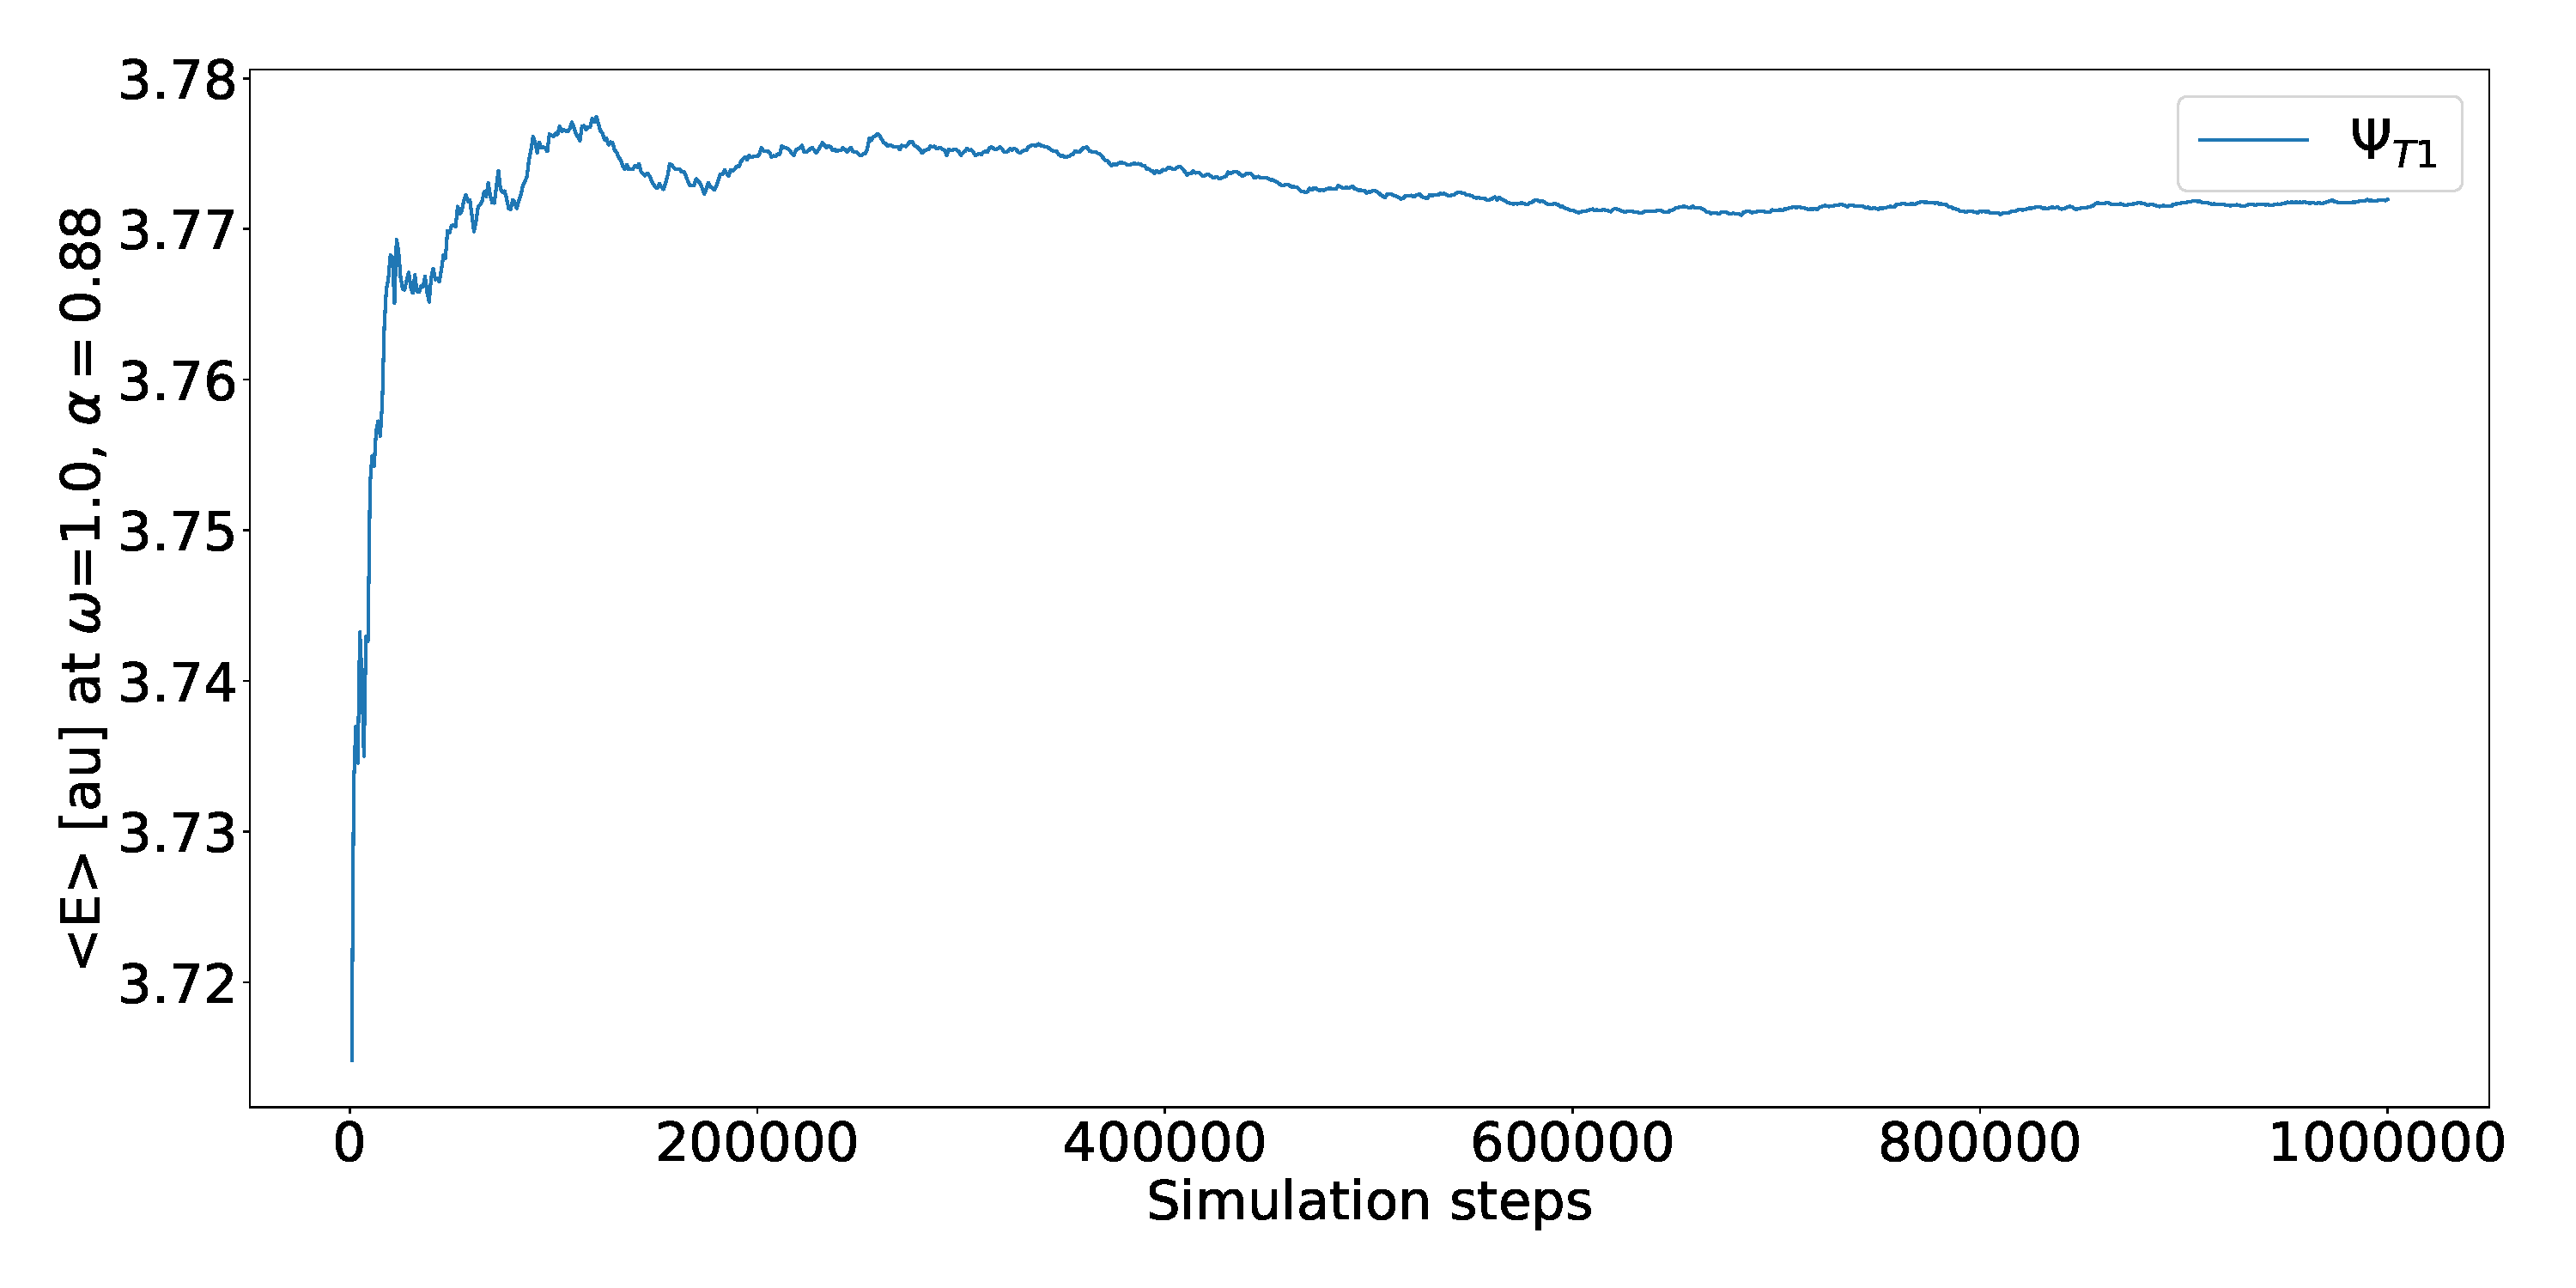
\includegraphics[width=\textwidth]{Energy_variation.pdf}
\caption[<E> as function of simulation steps]{$\braket{E}$ of $\Psi_{T1}$ as function of simulation steps for $\alpha$=0.88, $\omega=1.0$. Counting starts after a suitable value for the step size $dr$ has been found.}
\end{figure}
From that, we deduced that it takes roughly 200,000 simulation steps for the system to equilibrate. Depending on the initial guess of the step size $dr$, it takes some additional steps to find a suitable value for $dr$. Thus, we decided to discard 200,000 simulation steps before starting to sample, plus all the steps before a fitting $dr$ was found.
\subsection{Finding values for $\alpha$ and $\beta$ for $\Psi_{T2}$}
Finding right values for $\alpha$ and $\beta$ for $\Psi_{T2}$ is no easy task, as the ideal value, that is, the value yielding the lowest energy, of $\beta$ depends on the choice of $\alpha$. We developed an algorithm to find those values of beta and alpha that give the lowest energy. The requirement for the algorithm to work is that there exist no local minima, as these would be incorrectly recognized as the actual minimum, and that the amount of simulation steps is sufficient in order to ascertain that the average energies are calculated well enough and with a small enough standard deviation. 
The algorithm works as follows:\\
\IncMargin{1em}
\begin{algorithm}[H]  
\SetKwData{Left}{left}\SetKwData{This}{this}\SetKwData{Up}{up}
    Start with a guess for $\alpha$ and $\beta$\ and calculate $\braket{E}(\alpha,\beta$);
    $\Delta\alpha=\Delta\beta=0.1$\;
    \While{$\Delta\alpha>0.005$}{
        Calculate $\braket{E}(\alpha+\Delta\alpha,\beta$) and $\braket{E}(\alpha-\Delta\alpha,\beta$)\;
        \uIf{$\braket{E}(\alpha+\Delta\alpha,\beta)<\braket{E}(\alpha,\beta$)}{
            Continue "going to the right" and find the integer X such that $\braket{E}(\alpha+(X+1)\Delta\alpha,\beta)<\braket{E}(\alpha+X\cdot\Delta\alpha,\beta$)\;
            Update $\alpha=\alpha+X\cdot\Delta\alpha$\;
        }
        \uElseIf{$\braket{E}$($\alpha-\Delta\alpha ,\beta)<\braket{E}(\alpha ,\beta$)}{
            Continue "going to the left" and find the integer X such that $\braket{E}(\alpha-(X+1)\Delta\alpha,\beta)<\braket{E}(\alpha -X\cdot\Delta\alpha ,\beta $)\;
            Update $\alpha =\alpha -X\cdot\Delta\alpha $\;
        }
        Do exactly the same for $\beta$\;
        \uIf{$\alpha$ and $\beta$ remain unchanged}{
        Decrease $\Delta\alpha$ and $\Delta\beta =0.1$ to a tenth their original values.
        }
    }
\end{algorithm}
\DecMargin{1em}
In other words, $\alpha$ and $\beta$ are changed by a given step length until no lower energy is found  for that given step length. Then, the step length is decreased until the ideal values $\alpha$ and $\beta$ are found with two decimals accuracy. We also implemented some safeguards to make sure that $\alpha$ and $\beta$ always are positive.
\subsection{Unit Testing}
In order to test that the Monte Carlo sampling works as intended, unit tests were implemented. Because we know that $\Psi_{T1}$ is the correct wave function with $\alpha=1.0$ when the electron repulsion is ignored, we tested that the ground-state energy $\braket{E}$ is lowest (and equal to 3.0) for $\alpha=1.0$. We also tested that the standard deviation
\begin{equation}
\sigma_E^2 = \sqrt{\braket{E^2}-\braket{E}^2}
\end{equation}
is very small, and larger for other values of $\alpha$. \\
In addition, we tested that the virial theorem for the pure harmonic oscillator  $\braket{V}$= $\braket{T}$ holds true when the electron repulsion is ignored.
\section{Results}
\subsection{Results using $\Psi_{T1}$}
A visualisation of the average energy $\braket{E}$ and the standard deviation $\sigma$ for different values of $\omega$ can be found in figure \ref{function1_plot}. 
\begin{figure}[H]
\centering
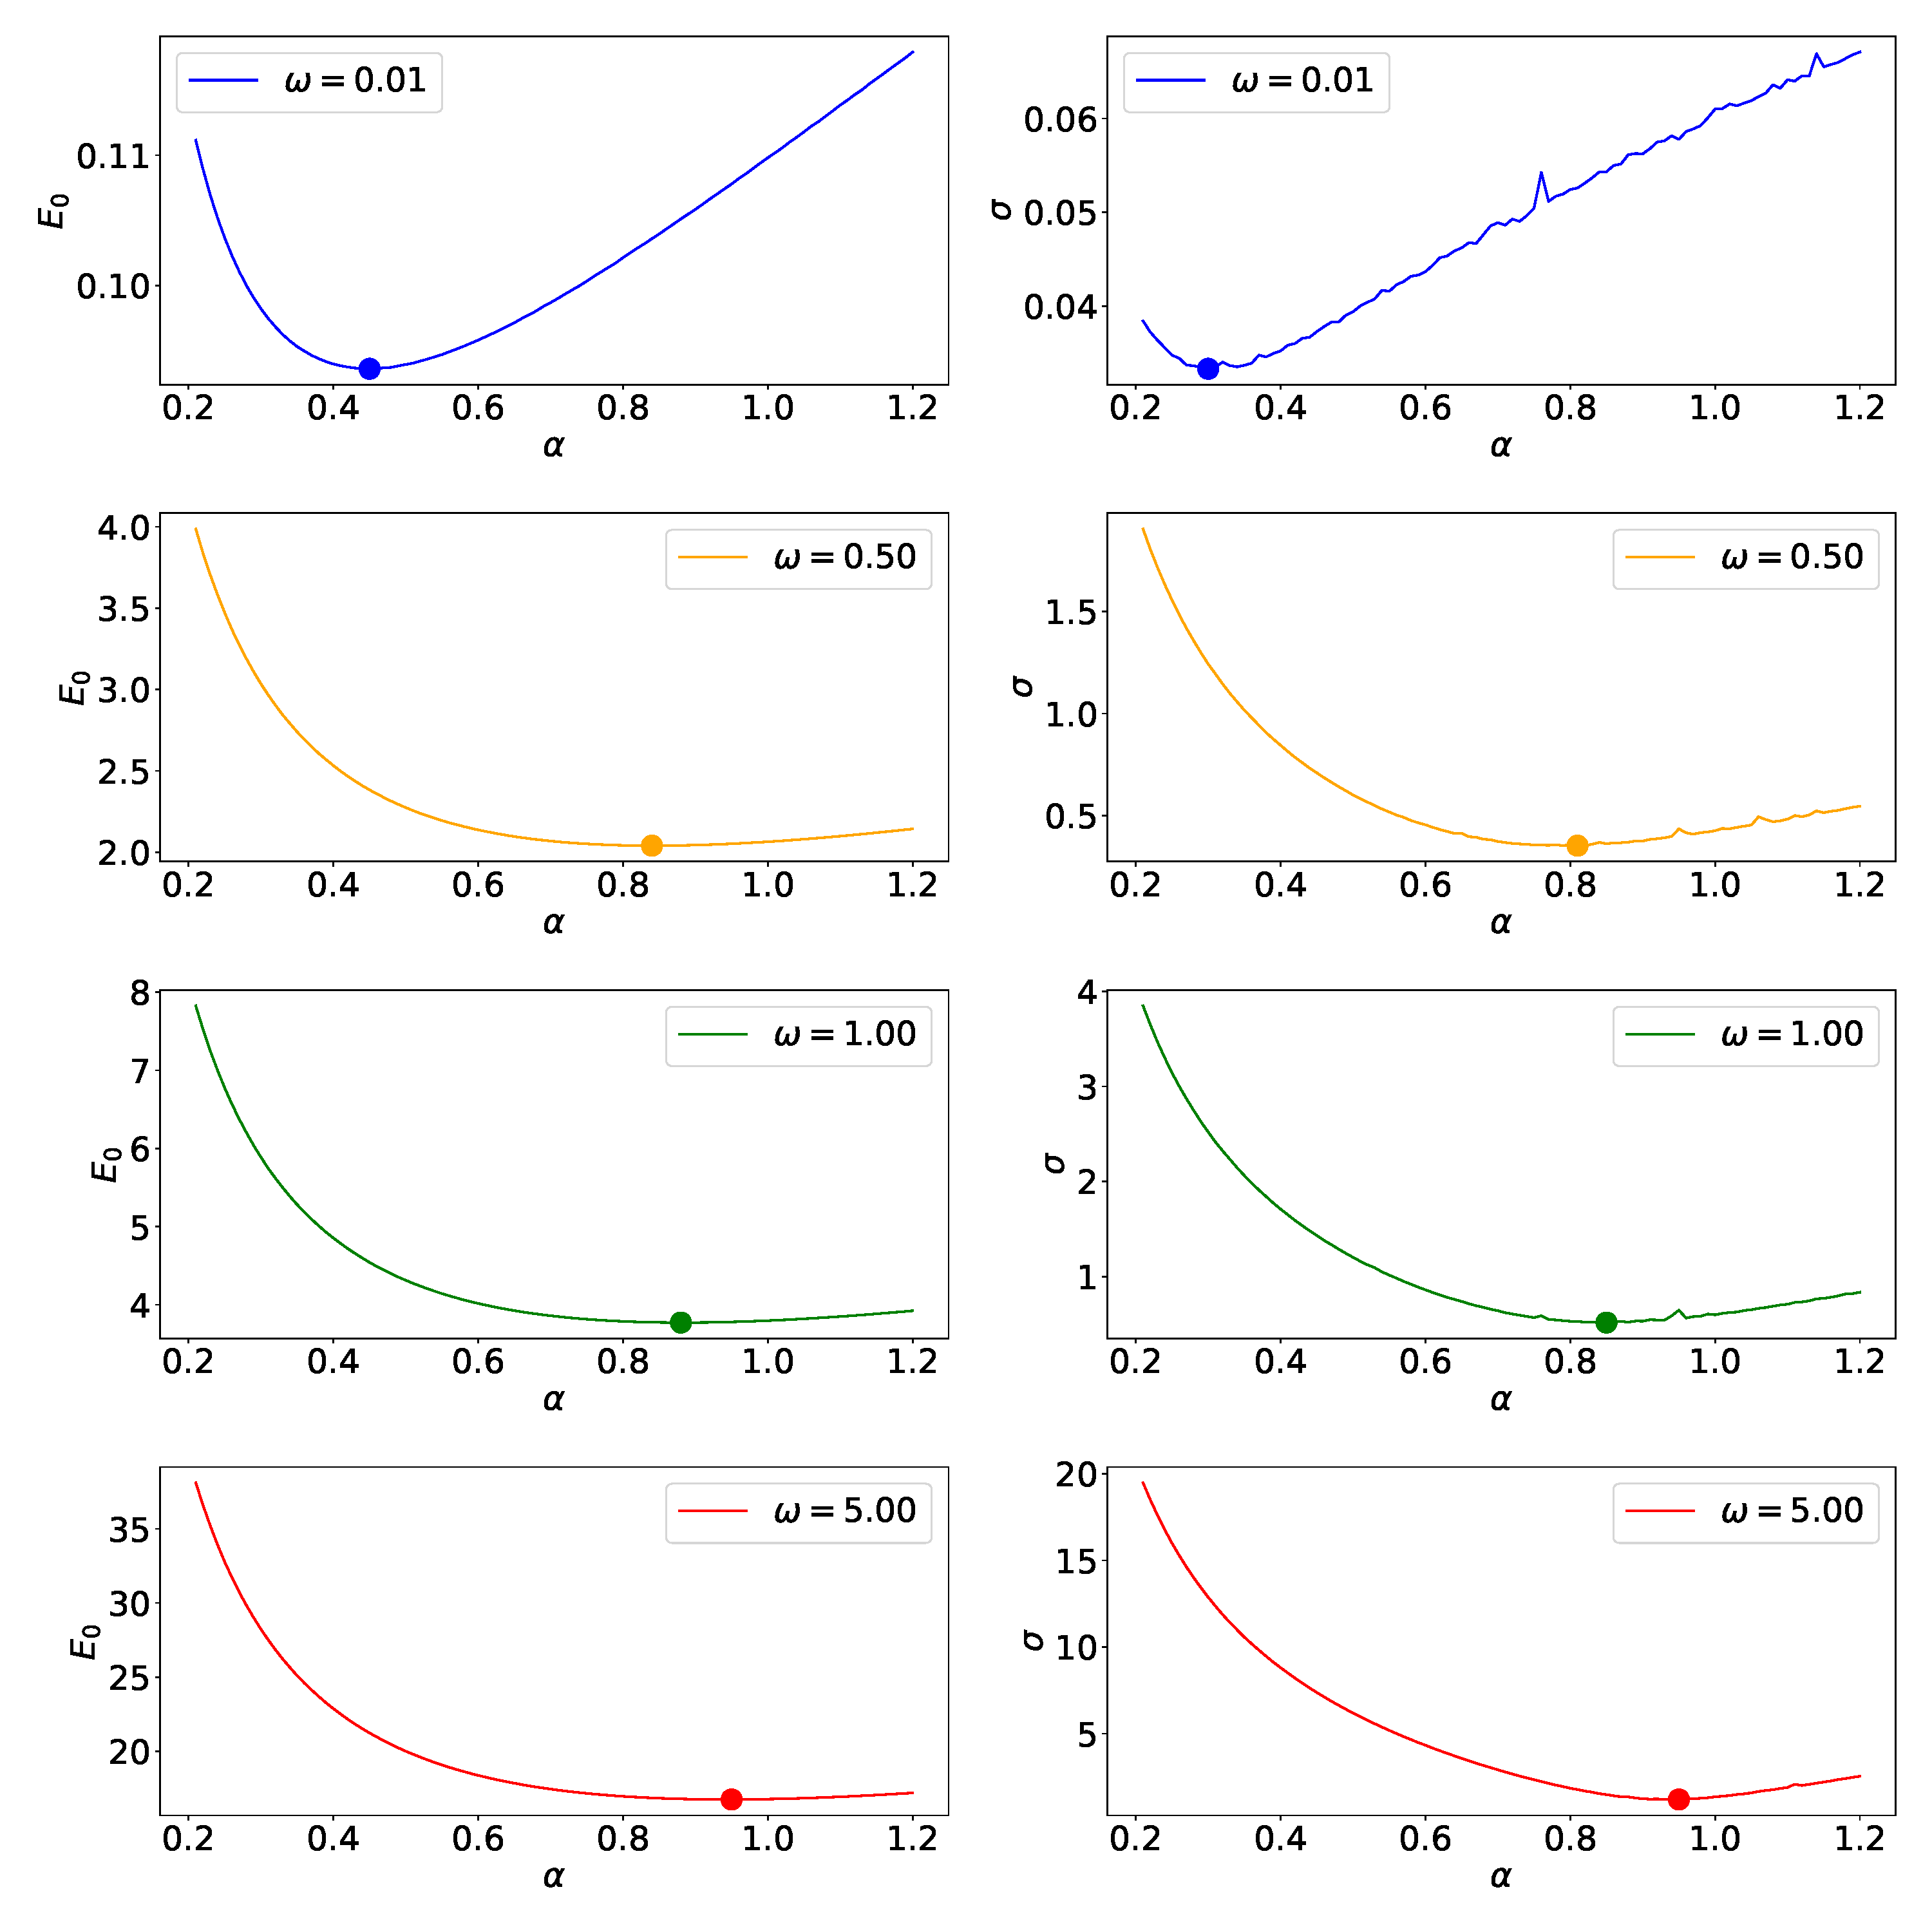
\includegraphics[width=\textwidth]{function1_plot.pdf}\label{function1_plot}
\caption[$\braket{E},\sigma$ as function of $\alpha$]{$\braket{E},\sigma$ as function of the variational parameter $\alpha$ for $\Psi_{T1}$ for $\omega\in\{0.01,0.5,1.0,5.0\}$ with $10^8$ Monte Carlo cycles}
\end{figure}
Table \ref{table1} contains information about several expectation values and the ideal value for $\alpha$ for the different values of $\omega$.
\begin{table}[H]
\centering
\caption[$\braket{E},\sigma$, $\alpha$ and $\braket{r_{12}}$]{$\braket{E},\sigma$, the $\alpha$ yielding the lowest result for  $\braket{E}$, and $\braket{r_{12}}$ for $\Psi_{T1}$ for $\omega\in\{0.01,0.5,1.0,5.0\}$ with $10^8$ Monte Carlo cycles}
\begin{tabular}{|l|l|l|l|l|}
\hline
                  & $\omega=0.01$ & $\omega=0.5$ & $\omega=1.0$ & $\omega=5.0$ \\ \hline
$\alpha$          & 0.45          & 0.84         & 0.88         & 0.95         \\ \hline
$\braket{E}$      & 0.0936        & 2.040        & 3.773        & 16.76        \\ \hline
$\sigma$          & 0.0373        & 0.3692       & 0.5206       & 1.204        \\ \hline
$\braket{r_{12}}$ & 23.78         & 2.462        & 1.701        & 0.733        \\ \hline
\end{tabular}\label{table1}
\end{table}
A lot of information can be extracted from this. For all values of $\omega$, one can see clearly that both the standard deviation and $\braket{E}$ have one single minimum. That is, there exists an unambiguous value for $\alpha$, yielding the lowest average energy or the lowest standard deviation. The values are different depending on $\omega$, which does not happen when the electron repulsion is ignored. Another observation is that the minima for $\braket{E}$ and $\sigma$ are not identical. This can be explained by the fact that the local energy is not the real ground state energy, because the trial wave function is not the real wave function. This leads to different integrals being evaluated for $\braket{E}$ and $\braket{E^2}$, and the minima coinciding would simply be a coincidence. Nevertheless, the ideal $\alpha$-value for the energy is similar to the lowest $\sigma$-value for the standard deviation. It is also interesting to see that the standard deviation for $\omega=0.01$ is in the same magnitude as $\braket{E}$ itself, while it is about one magnitude lower for $\omega=1.0$. A possible explanation is that the harmonic oscillator potential is that the electron repulsion dominates for very weak harmonic oscillator potentials, something that is not well incorporated in the wave function, so that the wave function's value is similar for quite different local energies. This is based on our earlier observation that the repulsion potential is a more severe "disturbance" for lower harmonic oscillator potentials.\\
The expectation value $\braket{r_{12}}$ for the distance between the two electrons decreases as $\omega$ increases, which makes sense - for lower values of  $\omega$, the electron repulsion dominates, and the particles stay far away from each other. 
\subsection{Varying $\alpha$ and $\beta$ for $\Psi_{T2}$}
The algorithm described above tries to find the best results for $\alpha$ and $\beta$. A typical "path" is shown (in chronological order) in table \ref{table2}, for the exemplary $\omega=0.7$. The results are similar when using different values of $\omega$.
\begin{table}[H]
\centering
\caption[Varying $\alpha$ and $\beta$]{The "path" gone by  $\alpha$ and $\beta$ yielding gradually lower results for  $\braket{E}$, as well as  $\braket{r_{12}}$ and $\sigma$ for $\Psi_{T2}$ for $\omega=0.7$ with $10^7$ Monte Carlo cycles}
\begin{tabular}{|l|l|l|l|l|}
\hline
$\alpha$ & $\beta$ & $\braket{E}$ & $\sigma$ & $\braket{r_{12}}$ \\ \hline
0.87     & 0.5     & 2.71342        & 0.138    & 2.23              \\ \hline
0.97     & 0.5     & 2.70880       & 0.111    & 2.11              \\ \hline
0.97     & 0.3     & 2.70227        & 0.032    & 2.20              \\ \hline
0.98     & 0.3     & 2.70226        & 0.032    & 2.19              \\ \hline
0.98     & 0.25    & 2.70172        & 0.019    & 2.22              \\ \hline
0.99     & 0.25    & 2.70162        & 0.014    & 2.21              \\ \hline
0.99     & 0.24    & 2.70160        & 0.014    & 2.22              \\ \hline
0.99     & 0.25    & 2.70160        & 0.015    & 2.21              \\ \hline
0.99     & 0.25    & 2.70162        & 0.014    & 2.21              \\ \hline
\end{tabular}\label{table2}
\end{table}
We see that the energy barely changes as soon as approximate values have been found, and that there is little room for improvement. However, the standard deviation decreases vastly when improving the parameters, and we see how energy reduction is correlated with reduction of $\sigma$, which seems to vary more intensely when varying $\alpha$ and $\beta$. This makes it feasible to find the lowest value for $\sigma$ instead of $\braket{E}$, however, it will not yield the lowest energy. It is also possible to see that $10^7$ Monte Carlo cycles simply is not enough to get reliable results, as the last row has an energy difference large enough to change the parameters $\alpha$ and $\beta$. However, using $10^7$ Monte Carlo cycles works nicely to get a general idea of the "true" lowest-energy parameters $\alpha$ and $\beta$, which we found are $\alpha=0.99$ and $\beta=0.24$.
\subsection{Results using $\Psi_{T2}$}
The results for different expectation values, and the optimal parameters $\alpha$ and $\beta$, are presented in table \ref{table3}. 
\begin{table}[H]
\centering
\caption[$\braket{E},\sigma$, $\alpha$,$\beta$ and  $\braket{r_{12}}$]{$\braket{E},\sigma$, the $\alpha$ and $\beta$ yielding the lowest result for  $\braket{E}$, and $\braket{r_{12}}$ for $\Psi_{T2}$ for $\omega\in\{0.01,0.5,1.0,5.0\}$ with $10^8$ Monte Carlo cycles. The right range for $\alpha$ and $\beta$ was found using the approach described above using $10^7$ simulation steps, and the values were confirmed and refined using  $10^8$ simulation steps. }

\begin{tabular}{|l|l|l|l|l|}
\hline
                  & $\omega=0.01$ & $\omega=0.5$ & $\omega=1.0$ & $\omega=5.0$ \\ \hline
$\alpha$          & 0.89          & 0.99         & 1.0          & 1.0          \\ \hline
$\beta$           & 0.05          & 0.14         & 0.27         & 0.59         \\ \hline
$\braket{E}$      & 0.0794        & 2.00         & 3.73         & 16.71        \\ \hline
$\sigma$          & 0.0020        & 0.012        & 0.017        & 0.034        \\ \hline
$\braket{r_{12}}$ & 28.69         & 2.68         & 1.81         & 0.758        \\ \hline
\end{tabular}\label{table3}
\end{table}

For all values of $\omega$ tested, $\braket{E}$ lies lower for $\Psi_{T2}$ than for $\Psi_{T1}$. The same observation can be made for the standard deviation $\sigma$. This shows that $\Psi_{T2}$ is a better approximation to the real wave function than $\Psi_{T1}$. For that reason, the expectation values from $\Psi_{T2}$ are, in general, more reliable than the ones gotten from $\Psi_{T1}$. However, this comes at the cost of having to find two non-independent parameters and increasingly complex expressions for both the function and the energy, making it more costly. 
A very interesting observation is the importance of the Jastrow factor. For smaller values of $\omega$, the relative decrease in energy is much higher than for larger values of  $\omega$: $\braket{E}$  using $\Psi_{T2}$ is 15\% lower than using $\Psi_{T1}$ for $\omega=0.01$, while we only have a difference of 1\% for $\omega=1.0$. This simply means that incorporating the electron repulsion becomes more important when the electron repulsion is the dominating force/potential. This makes sense, as $\Psi_{T1}$ is based on a wave function with no electron repulsion incorporated. We also see that $\sigma$ when using $\Psi_{T2}$ is less than a $10^th$ the size of the one using  $\Psi_{T1}$. This also indicates that the wave function $\Psi_{T2}$ is closer to the system's real wave function. \\
We make the same observation as for $\Psi_{T1}$ when it comes to the average electron distance $\braket{r_{12}}$, which decreases with an increasing energy, for the same reason. However, the values are slightly larger, thereby decreasing the potential energy, which also explains why $\Psi_{T2}$ yields better results.
\subsection{Comparison to the matrix diagonalization approach and analysis}
In an earlier numerical experiment conducted by us \cite{Project2}, we solved the same system numerically by finding its eigenvalues and eigenfunctions for the ground state and some excited states, using matrix diagonalisation. We also found the most likely distance between the two electrons. Table 4 repeats that information. 
\begin{table}[H]
\centering
\caption[Energies and distances compared to diagonalisation]{$\braket{E}$ and $r_{12}$ for $\Psi_{T1}$ and $\Psi_{T2}$, as well as the system's lowest eigenvalue and the most likely distance $r_{12,max}$. All quantities are in atomic units.}
\begin{tabular}{|l|l|l|l|l|l|l|}
\hline
$\omega$ & $\braket{E}(\Psi_{T1})$ & $\braket{E}(\Psi_{T2})$ & $E_0$ & $\braket{r_{12}}(\Psi_{T1})$ & $\braket{r_{12}}(\Psi_{T2})$ & $r_{12,max}$ \\ \hline
0.01     & 0.0936                 & 0.0794                  & 0.068 & 23.78                        & 28.69                        & 18.273    \\ \hline
0.5      & 2.040                  & 2.00                    & 1.87  & 2.462                        & 2.68                         & 1.667     \\ \hline
1.0      & 3.773                  & 3.73                    & 3.53  & 1.701                        & 1.81                         & 1.128     \\ \hline
5.0      & 16.76                  & 16.71                   & 16.22 & 0.733                        & 0.758                        & 0.471     \\ \hline
\end{tabular}
\end{table}
All approaches yield qualitatively similar results, as can be seen for $\omega=1.0$. The variational result using $\Psi_{T1}$ is 6\% larger than the analytical solution, which is 3.558 au, and still 5\% larger using $\Psi_{T2}$. However, that difference is too large to do more quantitative analysis on the system, no matter which trial wave function we use.  One advantage of the variational principle is that we always know that the energy we found is equal to or higher than the true ground state energy. We can see that the numerical solution approach yields much better results, but at least for $\omega=1.0$, the result is lower than the analytical solution. In general, this method gives no indication whether the real ground state energy is higher or lower, which is an advantage of the variational principle. We also see that the relative difference between all three approaches gets lower as $\omega$ is increased, which again reflects the fact that the electron repulsion gets less important for large values of $\omega$.\\
$r_{12,max}$ and $r_{12}$ are quite different and cannot be compared directly, because the real wave function is not symmetric, making the values nonidentical even for the same wave function. However, they scale similarly, and the same kind of observations can be taken from both. \\
One advantage of the variational principle is that it gives us an analytical (but wrong) expression for the wave function, making it, at least sometimes, possible to get analytical expressions for the local energy and other expectation values, as we did here. Nevertheless, the matrix diagonalisation approach yields much better results. This shows that solving problems as analytically as possible, pays off by giving better results, and is the preferred way of solving quantum mechanical problems, given it is possible.  
\subsection{Virial Theorem}
As stated above, for a pure harmonic oscillator, $\braket{V}=\braket{T}$. This relation does not hold true for systems where the electron repulsion is included. Figure \ref{Virial} plots $\braket{V}/\braket{T}$ for several values of $\omega$.
\begin{figure}[H]
\centering
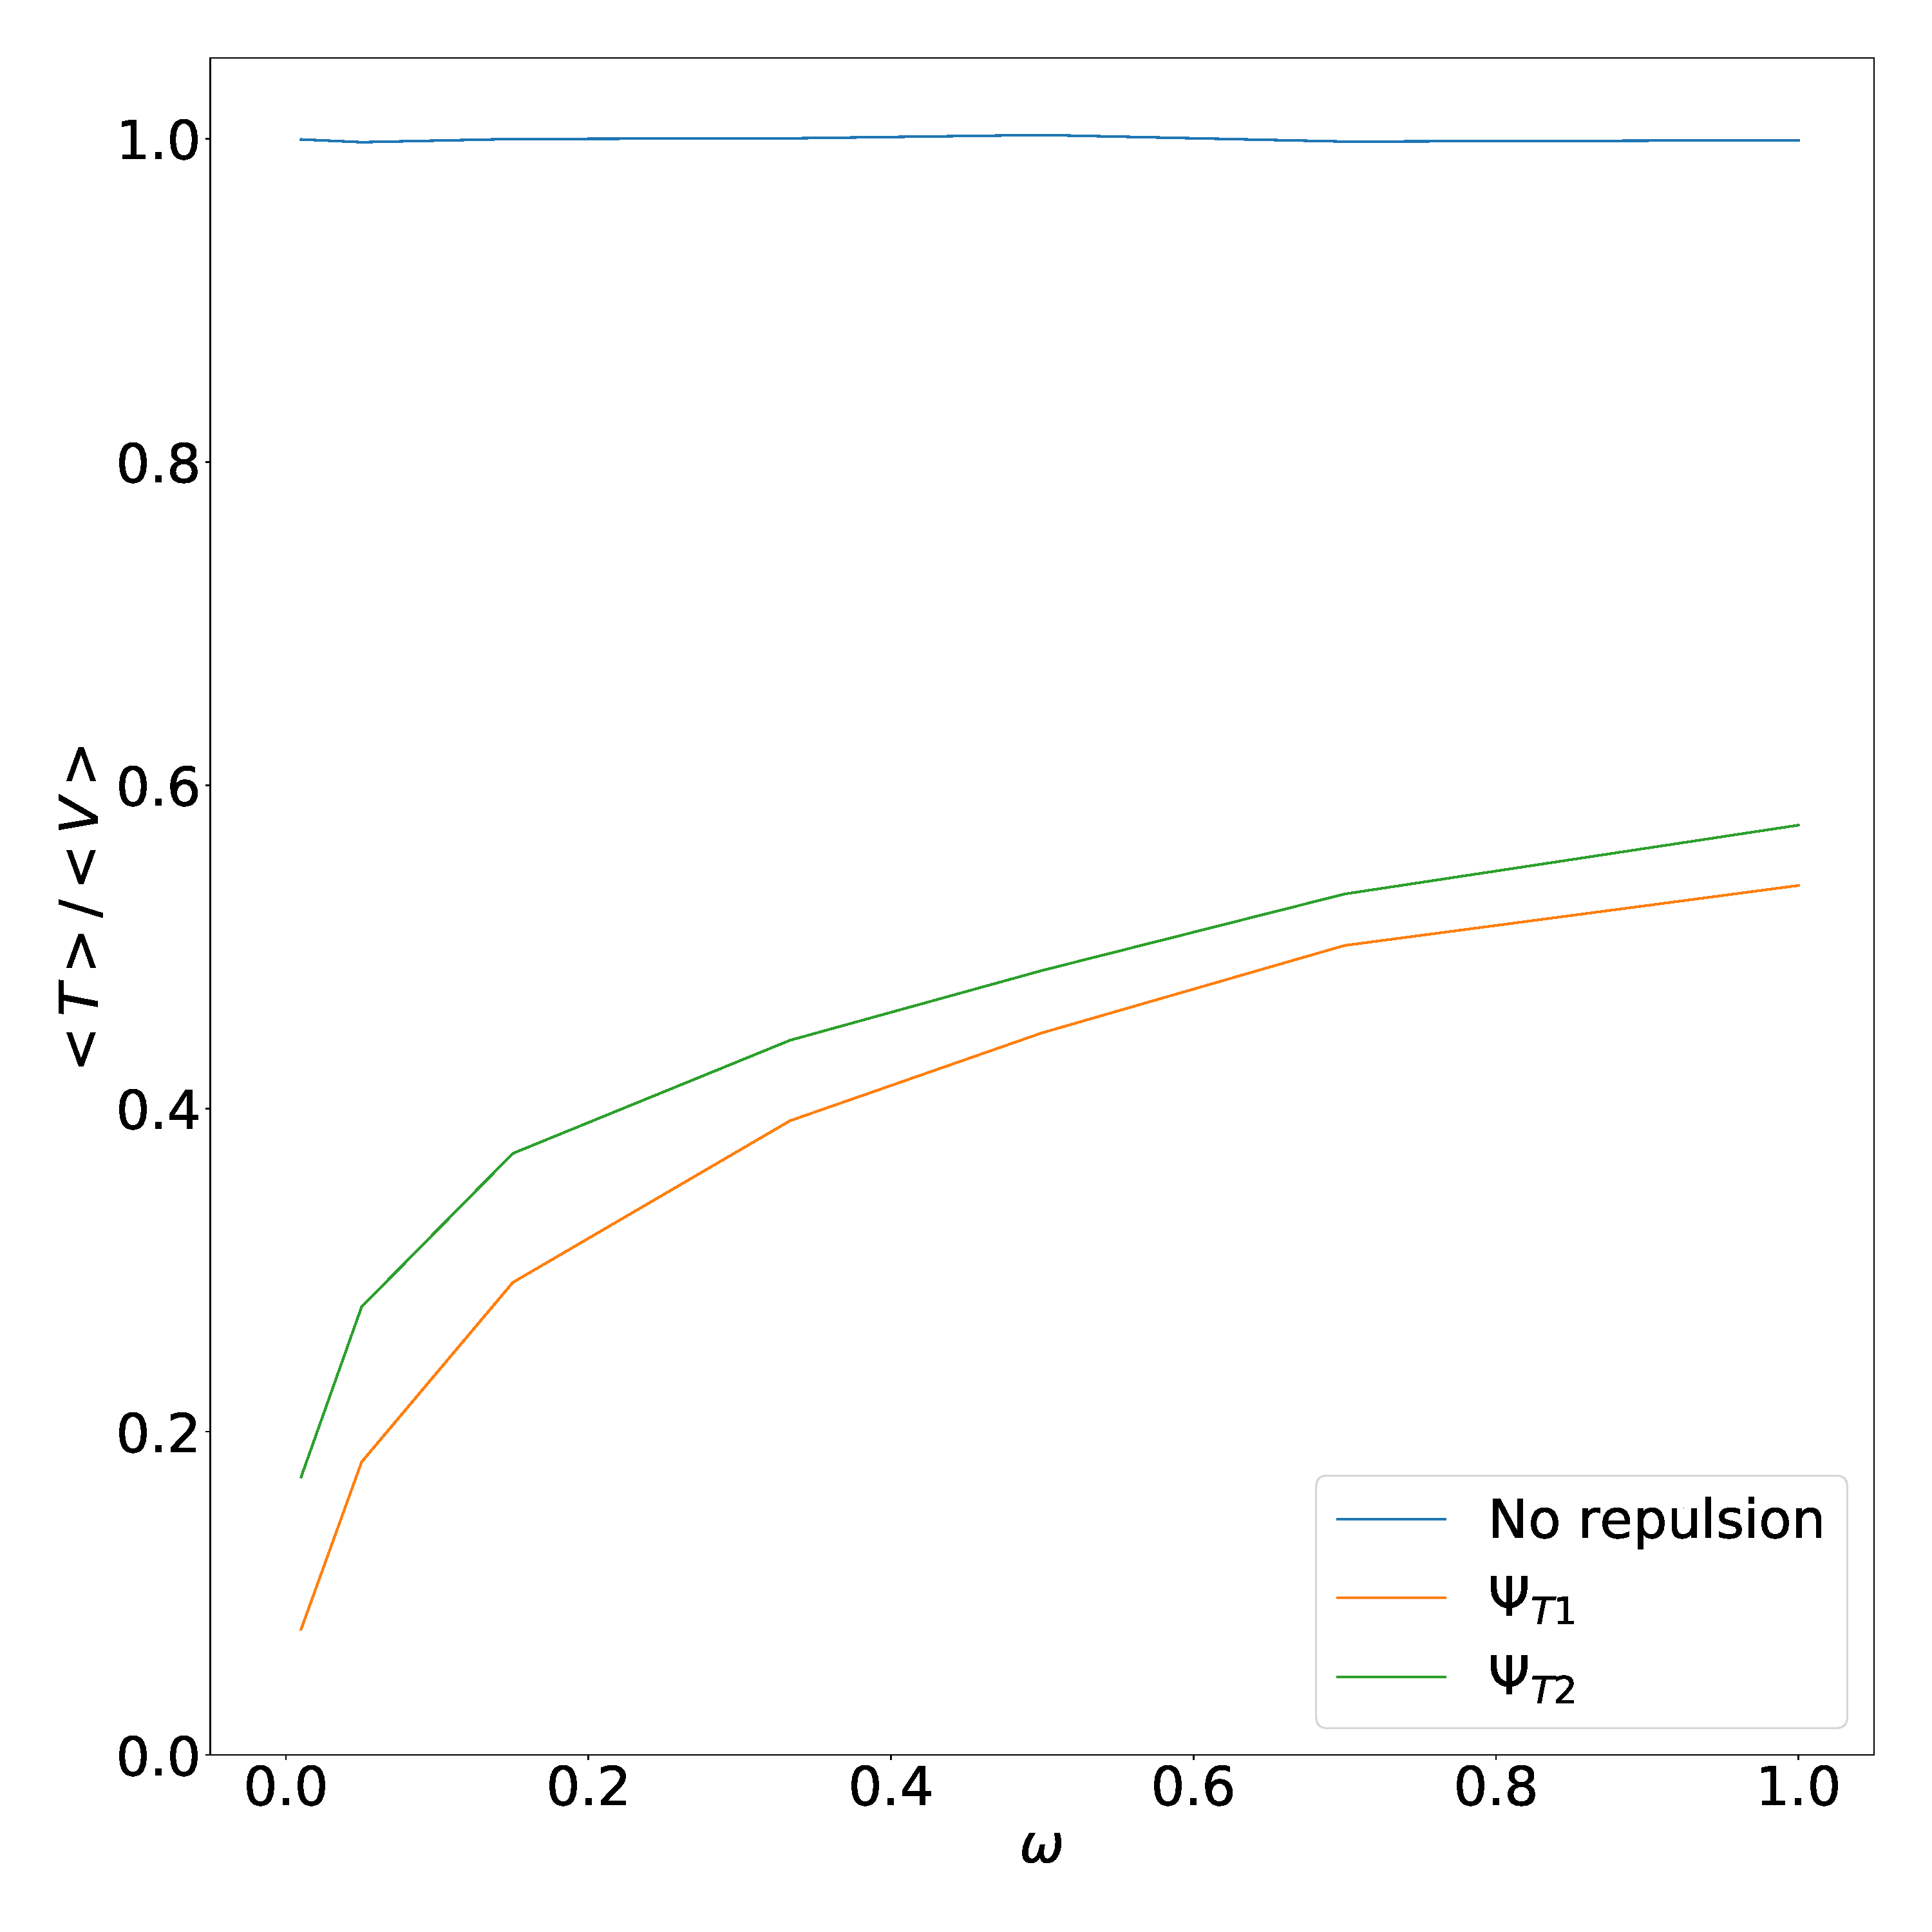
\includegraphics[width=0.7\textwidth]{Virial.pdf}\label{Virial}
\caption[$\braket{T}$/$0\braket{V}$ as function of $\omega$]{$\braket{T}$/$\braket{V}$ for different values of $\omega\in[0.01,1]$}
\end{figure}
This fits well with our earlier observations and explanations. Without electron repulsion, we see that $\braket{V}=\braket{T}$ holds true. However, with electron repulsion, $\braket{V}>\braket{T}$, but the difference gets smaller for increasing values of $\omega$. Again, this shows how the system starts resembling a harmonic oscillator more for larger values of $\omega$. The fact that $\braket{V}>\braket{T}$ also shows that the electron repulsion leads, relatively, to a decreased kinetic energy, an effect that is weaker for very strong harmonic potentials. It is very interesting to see that the quotient is larger using $\Psi_{T2}$ for all values, which can be related to the increased interelectronic distances. 
\section{Conclusion}
These simple simulations have shown that the variational theorem applied through Monte Carlo simulations is a feasible way to find the variationally lowest energy for a given wave function. Compared to values we found when we solved the system without approximations by solving the second derivative numerically, we managed to come as close as 15\% for very small values of $\omega$, and 5\% for larger values of $\omega$. Nevertheless, getting all the way down to the lowest energy, is no trivial task. Varying just two factors has not been enough, and reaching the real lowest energy wave function requires many more factors, something beyond the scope of this article. Despite not having the real wave function, we managed to replicate the qualitative observations from our earlier article. We also found that Monte Carlo simulation has the advantage that we can get many expectation values, such as $\braket{V}$, $\braket{E}$,$\braket{E^2}$ or $\braket{r_{12}}$, simply by evaluating extra functions while sampling. A clear advantage of using VMC methods for this class of quantum mechanical system is that conversion from Cartesian- to polar- coordinates is unnecessary. As opposed to the Jacobi eigenvalue algorithm, which for multiple- dimensional integrals become slow.\\The approaches taken here were rather simple, as the harmonic oscillator is a rather simple system, there was a function for the local energy, and, it was not necessary to pay closer attention to the Pauli principle, dealing with only two electrons in their singlet states. Varying through two parameters instead of one is no simple task, especially when the variational energies are quite close to one another. There is much room for improvement, and developing algorithms that manage finding minima with as few simulations as possible is crucial for larger systems.\\\\For the interacting system of electrons, the Jastrow factor has a diminishing effect on the energy of the system as $\omega$ increases. This is expected, as the kinetic energy of each electron will increase yielding more room for them to move in which ultimately means they spend less time in each others vicinity. For low values of $\omega$ however, the inclusion of the Jastrow factor lowered the energies expectation value by $15\%$ and so, for this system and especially systems with more electrons, closer together, the inclusion of this factor in the trial wave function will be essential to better approximations.\\\\The virial theorem was shown to hold for our model, both with and without electron- electron repulsion. In particular, the special case of the pure harmonic oscillator was proven and the proportionality constant $\alpha$ for
\begin{equation}
\braket{T} = \alpha \braket{V}
\end{equation}
was shown to increase as $\omega$ increases.
\section{Critique}

\section{Appendix}
\subsection{Proof of the variational principle in quantum mechanics}\label{Proof_variational_principle}
Given a normalized trial wave function $\ket{\psi}$. As any normalizable wave function can be expressed as a linear combination of energy eigenstates, we have that
$$
\ket{\psi} = \sum\limits_n C_n \ket{E_n}
$$
where $C_n$ is a complex coefficient, $\ket{E_n}$ is the energy eigenstate corresponding to the energy $E_n$ and $E_0=E_{gs}$. Now, calculating $\braket{H}$, 
$$
\braket{\psi|\hat{H}|\psi} = \sum\limits_{nm} \braket{E_m|C_m^*\hat{H}C_n|E_n}
$$
we get that 
$$
\braket{H}= \sum\limits_{nm} C_m^*C_n E_n \delta_{mn} =\sum\limits_{n} \big|  C_n \big|^2E_n
$$
where $\delta_{mn}$ is the Kronecker- delta.
\begin{equation}
\braket{H}=\sum\limits_{n} \big|  C_n \big|^2E_n \geq E_{gs}
\end{equation}
\begin{comment}
\subsection{Derivation of $E_{L2}$}
\begin{equation}
\nabla_i^2\Psi_{T2} = \nabla_i^2\left( \Psi_{T1}\exp{\left(\frac{r_{12}}{2(1+\beta r_{12})}\right)} \right)
\end{equation}
\[
\frac{d}{dr_i}\left(  \Psi_{T1}\exp{\left(\frac{r_{12}}{2(1+\beta r_{12})}\right)} \right) = \exp{\left(\frac{r_{12}}{2(1+\beta r_{12})}\right)}\frac{d}{dr_i}\Psi_{T1} + \Psi_{T1}\frac{d}{dr_i}\left( \exp{\left(\frac{r_{12}}{2(1+\beta r_{12})}\right)}\right)
\]
\begin{equation*}
\exp{\left(\frac{r_{12}}{2(1+\beta r_{12})}\right)}\frac{d}{dr_i}\Psi_{T1} = -\alpha \omega r_i\Psi_{T2}
\end{equation*}

\begin{equation*}
 \Psi_{T1}\frac{d}{dr_1}\left( \exp{\left(\frac{r_{12}}{2(1+\beta r_{12})}\right)}\right) = \frac{1}{4r_{12}\left( 1+\beta r_{12} \right)^2}  \Psi_{T1}\exp{\left(\frac{r_{12}}{2(1+\beta r_{12})}\right)} =  \frac{1}{4r_{12}\left( 1+\beta r_{12} \right)^2}\Psi_{T2}
\end{equation*}

\[
\frac{d}{dr_1}\Psi_{T2} = \left( \frac{1}{4r_{12}\left( 1+\beta r_{12} \right)^2} -\alpha \omega r_1\right)\Psi_{T2}
\]

\[
\frac{d}{dr_2}\Psi_{T2} = -\left( \frac{1}{4r_{12}\left( 1+\beta r_{12} \right)^2} +\alpha \omega r_2\right)\Psi_{T2}
\]

\[
\frac{d}{dr_1}\left( r_1^2 \frac{d}{dr_1}\Psi_{T2}\right) =  \frac{d}{dr_1}\left( r_1^2\left( \frac{1}{4r_{12}\left( 1+\beta r_{12} \right)^2} -\alpha \omega r_1\right)\Psi_{T2} \right)
\]

\[
= r_1^2\left( \frac{1}{4r_{12}\left( 1+\beta r_{12} \right)^2} -\alpha \omega r_1\right)^2\Psi_{T2}+\Psi_{T2} \frac{d}{dr_1}\left( r_1^2\left( \frac{1}{4r_{12}\left( 1+\beta r_{12} \right)^2} -\alpha \omega r_1\right)\right).
\]
\[
\frac{d}{dr_1}\left( r_1^2\left( \frac{1}{4r_{12}\left( 1+\beta r_{12} \right)^2} -\alpha \omega r_1\right)\right)=
\]
\[
\dfrac{r_1}{2r_{12}\left(\beta r_{12}+1\right)^2}-\dfrac{r_1^2}{8r_{12}^3\left(\beta r_{12}+1\right)^2}-\dfrac{\beta r_1^2}{4r_{12}^2\left(\beta r_{12}+1\right)^3}-3\alpha \omega r_1^2
\]

\[
\nabla_1^2\Psi_{T2} = \left( \left( \frac{1}{4r_{12}\left( 1+\beta r_{12} \right)^2} -\alpha \omega r_1\right)^2 +\dfrac{1}{2r_1r_{12}\left(\beta r_{12}+1\right)^2}-\dfrac{1}{8r_{12}^3\left(\beta r_{12}+1\right)^2}-\dfrac{\beta}{4r_{12}^2\left(\beta r_{12}+1\right)^3}-3\alpha \omega \right)\Psi_{T2}
\]
\\\\
\[
\frac{d}{dr_2}\left( r_2^2 \frac{d}{dr_2}\Psi_{T2}\right) =  \frac{d}{dr_2}\left( -r_2^2\left( \frac{1}{4r_{12}\left( 1+\beta r_{12} \right)^2} +\alpha \omega r_2\right)\Psi_{T2} \right)
\]
\[
= r_2^2\left( \frac{1}{4r_{12}\left( 1+\beta r_{12} \right)^2} +\alpha \omega r_2\right)^2\Psi_{T2} - \Psi_{T2}\frac{d}{dr_2}\left( r_2^2\left( \frac{1}{4r_{12}\left( 1+\beta r_{12} \right)^2} +\alpha \omega r_2\right) \right)
\]\\
\[
\frac{d}{dr_2}\left( r_2^2\left( \frac{1}{4r_{12}\left( 1+\beta r_{12} \right)^2} +\alpha \omega r_2\right) \right) = 
\]
\[
\dfrac{r_2}{2r_{12}\left(\beta r_{12}+1\right)^2}-\dfrac{r_2^2}{8r_{12}^3\left(\beta r_{12}+1\right)^2}-\dfrac{r_2^2\beta}{4r_{12}^2\left(\beta r_{12}+1\right)^3}+3\alpha \omega r_2^2
\]
\[
\nabla_2^2\Psi_{T2} = \left( \left( \frac{1}{4r_{12}\left( 1+\beta r_{12} \right)^2} +\alpha \omega r_2\right)^2 -   \dfrac{1}{2r_2r_{12}\left(\beta r_{12}+1\right)^2}+\dfrac{1}{8r_{12}^3\left(\beta r_{12}+1\right)^2}+\dfrac{\beta}{4r_{12}^2\left(\beta r_{12}+1\right)^3}-3\alpha \omega \right)\Psi_{T2}
\]

\[
\left( \nabla_1^2+\nabla_2^2 \right)\Psi_{T2} = \Bigg( \left( \frac{1}{4r_{12}\left( 1+\beta r_{12} \right)^2} +\alpha \omega r_2\right)^2 +\left( \frac{1}{4r_{12}\left( 1+\beta r_{12} \right)^2} -\alpha \omega r_1\right)^2- \cdots
\]
\[ 
\cdots \dfrac{1}{2r_{12}\left(\beta r_{12}+1\right)^2}\left( \frac{1}{r_1}-\frac{1}{r_2} \right)-6\alpha \omega \Bigg)\Psi_{T2}
\]

\end{comment}
\subsection{Figures}

\subsection{Tables}
\begin{table}[H]
\centering
\caption[$\alpha$ yielding the best $\braket{E}$ for given $\omega$]{$\alpha$ yielding the best $\braket{E}$ for given $\omega$ for $\Psi_{T1}$ for different values of $\omega$ with $10^8$ simulation steps }
\begin{tabular}{|l|l|l|l|l|l|l|l|l|}
\hline
$\omega$ & 0.01 & 0.05 & 0.15 & 1/3  & 0.5  & 0.7  & 1.0  & 5.0  \\ \hline
$\alpha$ & 0.45 & 0.63 & 0.74 & 0.81 & 0.84 & 0.87 & 0.88 & 0.95 \\ \hline
\end{tabular}
\end{table}
\begin{table}[H]
\centering
\caption[$\alpha$ and $\beta$ yielding the best $\braket{E}$ for given $\omega$]{$\alpha$ and $\beta$ yielding the best $\braket{E}$ for given $\omega$ for $\Psi_{T2}$ for different values of $\omega$ with $10^8$ simulation steps }
\begin{tabular}{|l|l|l|l|l|l|l|l|l|}
\hline
$\omega$ & 0.01 & 0.05 & 0.15 & 1/3  & 0.5  & 0.7  & 1.0  & 5.0  \\ \hline
$\alpha$ & 0.89 & 0.95 & 0.98 & 0.99 & 0.99 & 0.99 & 1.00 & 1.00 \\ \hline
$\beta$ & 0.05 & 0.09 & 0.13 & 0.14 & 0.17 & 0.24 & 0.27 & 0.59 \\ \hline

\end{tabular}
\end{table}

\subsection{List of programs}\label{Listofprograms}
All programs can be found on \url{https://github.com/adrian2208/FYS3150_collab} in the folder "Project5".


\begin{itemize}
\item[1.] b.cpp - Program with several options of writing to file, different matrices etc., for a given temperature and lattice size
\item[2.] e\_not\_parallel.cpp - Like b, but can run over several lattices and temperatures, more efficient
\item[3.] e.cpp - Same as above, but parallelized with openMPI
\item[4.] vecop.hpp - Several functions
\item[5.] vecop.cpp - Functions, out of which some are used.
\item[6.] tests\_main.cpp - Unit testing.
\item[7.] a.py - Analytical solution. Not properly up to date!
\item[8.] plot\_cv.py - Creates $2\times2$ plot for the larger simulations, also calculates $T_C(L_{\rightarrow \infty})$
\item[9.] plot\_distribution.py Plots the distribution histograms at different temperatures.
\item[10.] plot\_energy\_simulation\_step.py Plots the  avg. energy, the avg. magnetisation and the amount of accepted steps as a function of simulation step.
\item[11.] functions.hpp \& functions.cpp - Contains functions for parallelization, and all the integrands, and some more.
\end{itemize}

\bibliographystyle{Plain}



\bibliography{citations}



\begin{comment}

$$
\begin{bmatrix}
0 & 0 & 0 & 0 \\
0 & 0 & 0 & 0 \\
0 & 0 & 0 & 0 \\
0 & 0 & 0 & 0 \\
\end{bmatrix}
$$

\begin{lstlisting}[caption=insert caption]
for (unsigned int i = 0; i<100;i++{
}
\end{lstlisting}

\begin{figure}[h]
\includegraphics[width=8cm]{}
\caption{include caption}
\end{figure}

\end{comment}

\end{document}